%! Author = lazza
%! Date = 28/05/2022

\section{Multiprocessors}\label{sec:multiprocessors}
Till now we considered single cores architectures and how to increase the ILP in(side) such architectures.

\begin{figure}[h]
    \centering
    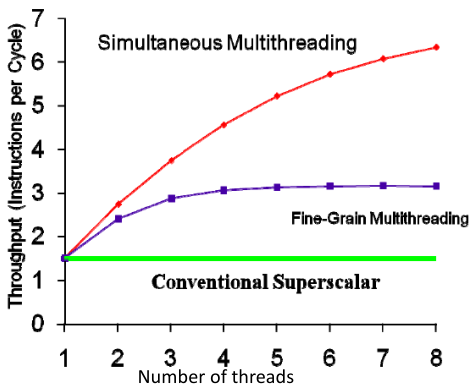
\includegraphics[scale = 0.4]{images/superscalar-vs-multithreading}
    \caption{Superscalar vs multithreading}
    \label{fig:superscalar-vs-multithreading}
\end{figure}

\paragraph{Beyond ILP}
We have seen the superscalar architecture, which can issue multiple instructions per clock cycle but these systems are
very complex to design and the returns are diminishing.
Another step forward towards parallelism is adding multithreading (or multiprocess) support to our single cores, but
the throughput of such systems reach their limits soon in terms of number of threads, what if we are willing to
have much more threads running?
Can we increase our throughput and support large-scale parallel systems?

\paragraph{Physical limitations}
\begin{itemize}
    \item difficult to increase performance and clock frequency of the single core
    \item a deep pipeline:
    \begin{itemize}
        \item heat dissipation
        \item speed light transmission problems in wires
        \item difficulties in design and verification
        \item requirement of very large design groups (higher complexity)
    \end{itemize}
\end{itemize}

Designing faster architectures may lead to worse throughput than running in parallel existing architectures;
furthermore, the design of a new architecture takes more time and cost.
Replication of cores doesn't come for free, to connect multiple microprocessor in a complex system we have to implement
some communication policies between cores.

\paragraph{Communication architecture} requires:
\begin{itemize}
    \item abstractions (HW/SW interfaces)
    \item different structures to realize abstraction efficiently
\end{itemize}

\subsection{Parallel architectures}\label{subsec:parallel-architecture}
\textit{“A parallel computer is a collection of
processing elements that cooperates and
communicate to solve large problems fast”}\footnote{Almasi and Gottlieb, Highly Parallel Computing, 1989}

\subsubsection{SISD}
A serial (non-parallel) computer with deterministic execution, i.e., the architectures seen till now, the oldest and
most common type of computer.
\begin{figure}[h]
    \centering
    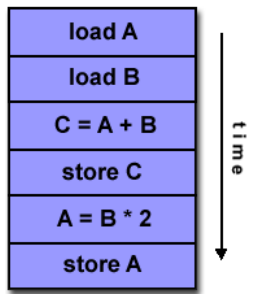
\includegraphics[scale = 0.3]{images/sisd}
    \caption{SISD}
    \label{fig:sisd}
\end{figure}

\subsubsection{MISD}
Another parallel computer, where a single data stream is fed into multiple processing units.
Each processing unit operates on the data independently via independent instruction streams.
Niche use cases such as regex expressions.
\begin{figure}[H]
    \centering
    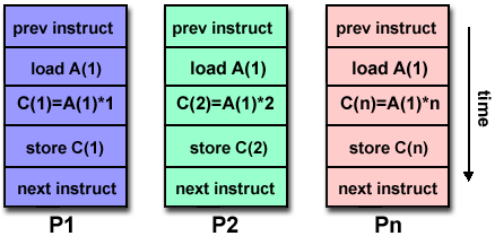
\includegraphics[scale = 0.3]{images/misd}
    \caption{MISD}
    \label{fig:misd}
\end{figure}

\subsubsection{SIMD}
A type of parallel computer, where all processing units execute the same instruction at any given clock cycle, each
one operates on a different data stream.
Data pipelining into processing unit, useful for example for operations on matrices.
Best suited for specialized problems characterized by a high degree of regularity, such as graphics/image processing
(GPUs) or machine learning.
Processors are typically special-purpose.
There is only one single instruction memory and control processor to fetch and dispatch instructions.

\begin{figure}[H]
    \centering
    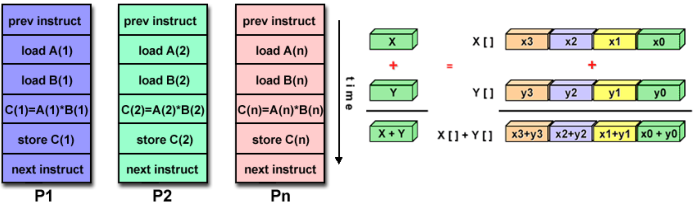
\includegraphics[scale = 0.3]{images/simd}
    \caption{SIMD}
    \label{fig:simd}
\end{figure}

A central controller broadcasts instructions to
multiple processing elements (PEs):
\begin{itemize}
    \item only requires one controller for whole array
    \item only requires storage for one copy of program
    \item all computations are fully synchronized
\end{itemize}

\begin{figure}[H]
    \centering
    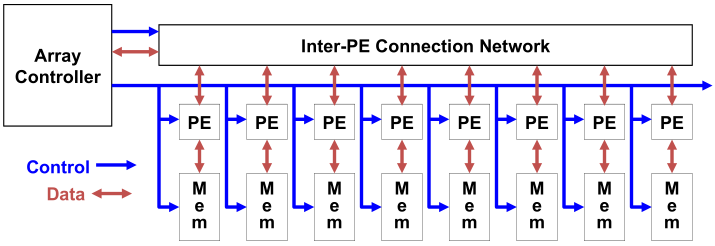
\includegraphics[scale = 0.3]{images/simd-scheme}
    \caption{SIMD scheme}
    \label{fig:simd-scheme}
\end{figure}

\begin{itemize}
    \item[\textrightarrow] Synchronized units: single Program Counter
    \item[\textrightarrow] Each unit has its own addressing registers\\
    – Can use different data addresses
    \item[\textrightarrow] Motivations for SIMD:\\
    – Cost of control unit shared by all execution units\\
    – Only one copy of the code in execution is necessary
    \item[\textrightarrow] Real life:\\
    – SIMD have a mix of SISD instructions and SIMD\\
    – A host computer executes sequential operations\\
    – SIMD instructions sent to all the execution units, which
    has its own memory and registers and exploit an
    interconnection network to exchange data
\end{itemize}

\paragraph{Alternative Model: Vector Processing}
Although being similar to SIMD, cannot be categorized under the Flynn's taxonomy.
SIMD instruction sets lack crucial features when compared to vector processor instruction sets, the most important of
these is that vector processors, inherently by definition and design, have always been variable-length since their
inception.

Vector processors have high-level operations that work on linear arrays of numbers: "vectors".
A vector processor consists of a pipelined scalar unit (may be out-of order or VLIW) plus a vector unit.

Styles of vector architectures:
\begin{itemize}
    \item \textit{memory-memory vector processors:} all vector
    operations are memory to memory
    \item \textit{vector-register processors:} all vector operations between vector registers (except load and store)
    , vector equivalent of load-store architectures
\end{itemize}

\begin{figure}[h]
    \centering
    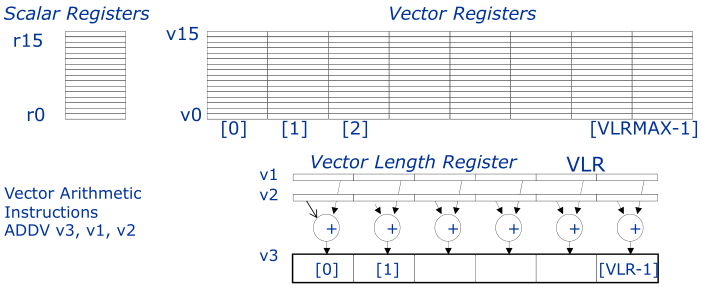
\includegraphics[scale = 0.35]{images/vector-programming-model}
    \caption{Vector programming model}
    \label{fig:vector-programming-model}
\end{figure}

\begin{table}[h]
    \begin{verbatim}
                # C code
                for (i=0;i<64; i++)
                C[i] = A[i]+B[i];
    \end{verbatim}
    \begin{tabular}{p{1.6in}|p{1.4in}}
        \begin{verbatim}
    # Scalar Code
    LI R4, #64
    loop:
    L.D F0, 0(R1)
    L.D F2, 0(R2)
    ADD.D F4, F2, F0
    S.D F4, 0(R3)
    DADDIU R1, 8
    DADDIU R2, 8
    DADDIU R3, 8
    DSUBIU R4, 1
    BNEZ R4, loop
        \end{verbatim} &
        \begin{verbatim}
    # Vector Code
    LI VLR, #64
    LV V1, R1
    LV V2, R2
    ADDV.D V3,V1,V2
    SV V3, R3
        \end{verbatim}
    \end{tabular}
    \label{tab:vector-programming-comparison}
\end{table}

add stuff from slide +\\
vector registers, more area more cost and more energy\\
vector machina distance between functional units can be bottleneck, use 3d structure.\\
situation: tons of data that we want to study\\

\textbf{Sony Playstation 2000:} a system running in parallel a MIPS cpu for I/O together with parallel
vector processors for image pre-processing.
\begin{figure}[h]
    \centering
    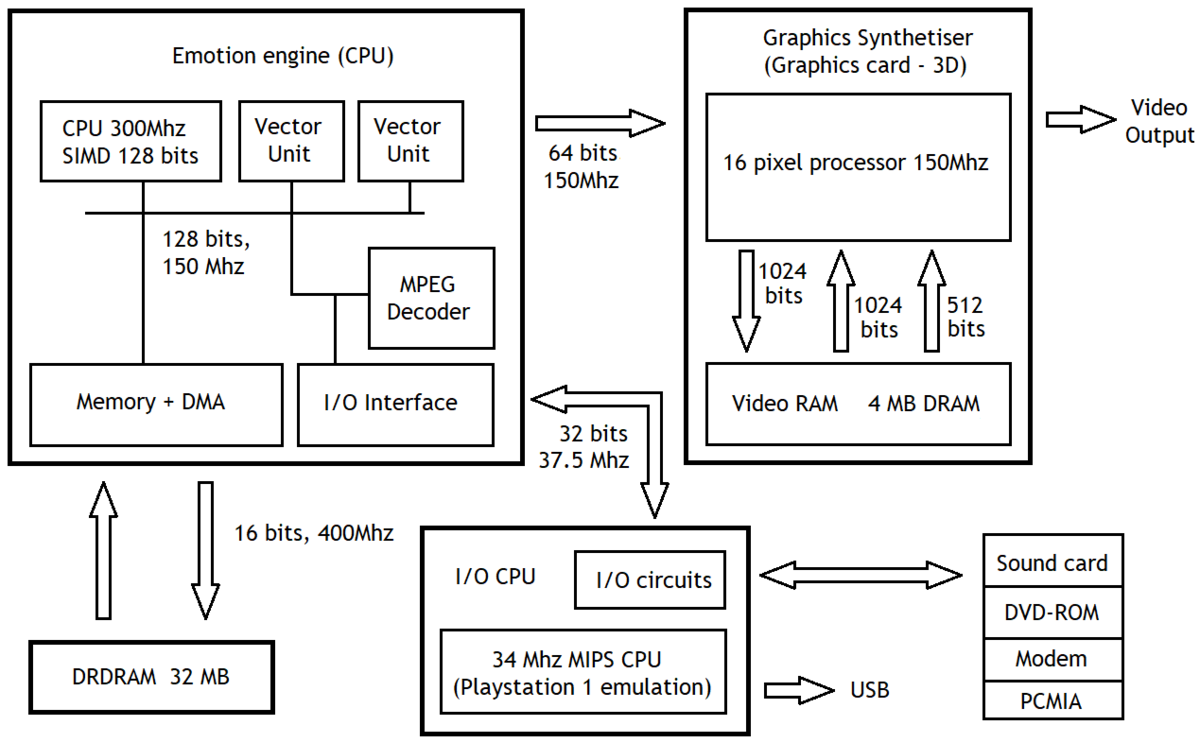
\includegraphics[scale = 0.2]{images/sony-playstation-2000}
    \caption{Sony Playstation 2000 architecture}
    \label{fig:sony-playstation}
\end{figure}

\subsubsection{MIMD}
The most common parallel computer nowadays, every processor may have a different instruction and data stream.
See chapter~\ref{sec:mimd}.
